%! Author = JustinMa
%! Date = 5/19/25

% Preamble
\documentclass[12pt]{article}


% Packages
\usepackage{amsmath}
\usepackage{graphicx}
\usepackage{booktabs}
\usepackage{caption}
\usepackage{float}
\usepackage{tikz}
\usepackage{setspace}

\doublespacing
\usetikzlibrary{shapes.geometric, arrows.meta, positioning}

\tikzstyle{layer} = [rectangle, draw=black, minimum width=5cm, minimum height=1cm, text centered, text width=5cm]
\tikzstyle{arrow} = [thick, -{Stealth}]

% Document
\usepackage{times}
\begin{document}

    \centerline{\textbf{Investigating Overfitting in Convolutional Neural Networks}}

    \noindent\textbf{1. Introduction}

    Neural networks are a form of machine learning models, roughly inspired from how the human brain processes information.
    They have become increasingly prevalent in our developing world, providing powerful and unique solutions to a wide variety of problems.
    However, with power also comes risk, as training a neural network too much can cause overfitting.
    Overfitting occurs when a model learns the training data too well and performs poorly on unseen data.
    In this study, we investigate whether increasing the number of parameters in a convolutional neural network
    leads to greater overfitting, as measured by the difference between training and test accuracy.

    \noindent\textbf{2. Statistical Question}

    Does increasing the number of parameters in a fixed CNN architecture cause a greater difference between training and testing accuracy?

    \noindent\textbf{Hypotheses}\newline
    $H_0: \beta = 0$ \newline
    $H_a: \beta \geq 0$
    \newline \newline
    Where $\beta$ is the true slope of the population least-squares regression line that relates number of parameters of the model to the difference in accuracy of the model on the train dataset and the test dataset.

    \noindent\textbf{3. Data Collection}

    We trained $\mathbf{x}$ convolutional models on a randomly selected small subset of size 100 images from the CIFAR-10 dataset, each with the same architecture (\textit{see figure 1}).
    Each model had a different number of parameters, uniformly ranging from approximately 1 million to 50 million.

    % Model Architecture
    \noindent\textbf{Model Architecture}
    \begin{center}
        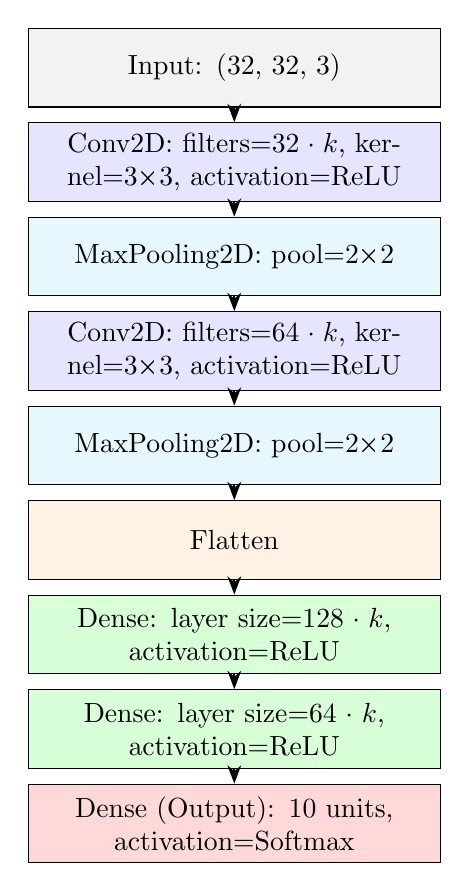
\begin{tikzpicture}[node distance=1.2cm]

            \node (input) [layer, fill=gray!10] {Input: (32, 32, 3)};
            \node (conv1) [layer, fill=blue!10, below of=input] {Conv2D: filters=$32\cdot k$, kernel=3×3, activation=ReLU};
            \node (pool1) [layer, fill=cyan!10, below of=conv1] {MaxPooling2D: pool=2×2};
            \node (conv2) [layer, fill=blue!10, below of=pool1] {Conv2D: filters=$64\cdot k$, kernel=3×3, activation=ReLU};
            \node (pool2) [layer, fill=cyan!10, below of=conv2] {MaxPooling2D: pool=2×2};
            \node (flatten) [layer, fill=orange!10, below of=pool2] {Flatten};
            \node (dense1) [layer, fill=green!15, below of=flatten] {Dense: layer size=$128\cdot k$, activation=ReLU};
            \node (dense2) [layer, fill=green!15, below of=dense1] {Dense: layer size=$64\cdot k$, activation=ReLU};
            \node (output) [layer, fill=red!15, below of=dense2] {Dense (Output): 10 units, activation=Softmax};

            \draw [arrow] (input) -- (conv1);
            \draw [arrow] (conv1) -- (pool1);
            \draw [arrow] (pool1) -- (conv2);
            \draw [arrow] (conv2) -- (pool2);
            \draw [arrow] (pool2) -- (flatten);
            \draw [arrow] (flatten) -- (dense1);
            \draw [arrow] (dense1) -- (dense2);
            \draw [arrow] (dense2) -- (output);

        \end{tikzpicture}
    \end{center}

    \centerline{\textit{Figure 1: Architecture of CNN Model}}

    \noindent\textbf{Data Display}


    \noindent\textbf{Data Analysis}

    \noindent\textbf{Conclusion}

    \noindent\textbf{Reflection}
\end{document}